\documentclass[11pt,a4paper,DIV=11]{scrlttr2}
\usepackage[T1]{fontenc}
\usepackage{fontspec}
\setmainfont{Arial}
\usepackage[utf8]{inputenc}
\usepackage{lmodern}
\usepackage{graphicx}
\usepackage{color}
\usepackage{url}
\usepackage{amssymb}
\usepackage{fancyhdr}
\usepackage{hyperref}
%\usepackage{showframe}

\usepackage[british,UKenglish,english]{babel}

\LoadLetterOption{DIN}

\setlength{\parindent}{0em}

\KOMAoptions{
    foldmarks=false,
    addrfield=false,
    fromalign=right,
    fromrule=aftername,
    footsepline=off,
    fromurl=false,
    fromemail=false,
    firstfoot=false,
}

\rhead{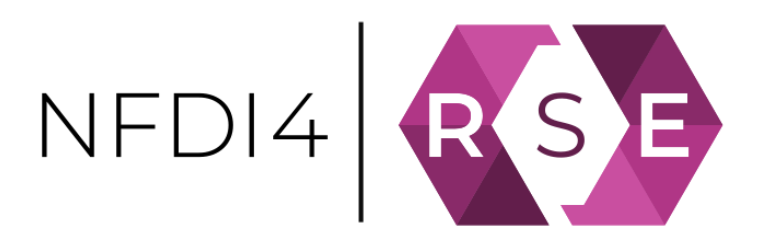
\includegraphics[height=2em]{nfdi4rse_logo.png}}
\pagestyle{fancy}

\definecolor{col_deRSE}{rgb}{0.535, 0.164, 0.410}

\setkomavar{fromname}{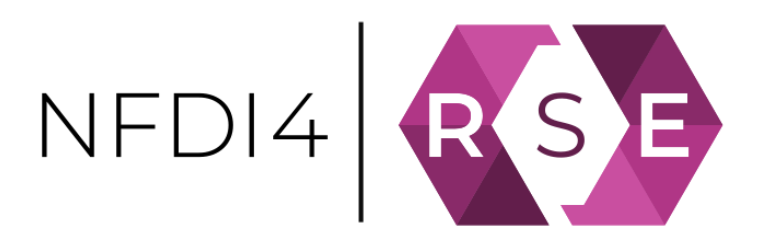
\includegraphics[height=1em]{nfdi4rse_logo.png}}
\setkomafont{fromrule}{\color{col_deRSE}}
\setkomavar{date}{}

\begin{document}

\newcommand{\mysec}[1]{\textbf{\hspace{-1cm}#1}\\}

\setkomavar{subject}{}

\begin{letter}{}

\begin{centering}
\textbf{\large
NFDI4RSE:\\National Research Data Infrastructure for Scientific Software\\*[1em]
Non-binding letter of intent for the NFDI\\*[2em]
}
\end{centering}

\mysec{1. Binding letter of intent as advance notification or non-binding letter of intent}

$\boxtimes$ Non-binding letter of intent (anticipated submission in 2020)\\

\mysec{2. Formal details}

\textbf{Planned name of the consortium:}\\

National Research Data Infrastructure for Scientific Software\\
(Nationale Forschungsinfrastruktur für wissenschaftliche Software)\\

\textbf{Acronym of the planned consortium:}\\

NFDI4RSE (formerly RSE4NFDI)\\

\textbf{Applicant institution}\\

Friedrich Schiller University Jena\\
Fürstengraben 1\\
07743 Jena\\

\textbf{Spokesperson}\\

Dr. Frank Löffler\\
Department for Mathematics and Computer Science\\
Friedrich Schiller University Jena\\
07743 Jena\\
\href{mailto:nfdi4rse-orga@de-rse.org}{nfdi4rse-orga@de-rse.org}\\

\clearpage
\mysec{3. Objectives, work programme and research environment}

\textbf{Research area of the proposed consortium (according to the DFG classification system)}\\

44 - Computer Science, Systems and Electrical Engineering\\

\textbf{Concise summary of the planned consortium’s main objectives and task area}\\

All scientific domains are currently facing a massive and conspicuous increase of observational data through increasingly digitised scientific workflows. Research software, with its key capabilities to operationalise, repeat, disseminate and document analytical procedures, has become one of the pillars of science in general. Usable and  sustainable open software is a prerequisite for reproducible research. However, in contrast to scholarly communication and primary data sets, research software has long been considered to be a mere tool, or a second-class research product at most.

Software is often treated as “data”, i.e. a static digital object. While some aspects of software can indeed be handled this way, good practices for data fail to address numerous central properties of software and its development process: (1)~Software requires maintenance in order to ensure its continuous usability in permanently changing hardware and software environments. (2)~Due to necessary adaptations and continuous development, software usually evolves over time. (3)~Such modifications will often - especially after the initial publication and successful adoption - come from external contributors. These desirable collaborations raise questions about acknowledgement, accountability and copyright. (4)~While software projects have typically low requirements in terms of storage space, they critically depend on fine-grained change histories, version management, collaborative online platforms, and a scalable computational infrastructure for testing. (5)~Most software builds on existing libraries or frameworks, which also change over time, thereby creating dependencies on a specific version. Therefore, long-term sustainability can only be achieved by taking these dependency graphs into account. (6)~Software can be conveyed as source code or compiled binaries, leading to more complex licensing conditions. These interconnected - and often neglected - properties necessitate a distinct treatment of software to advance it to a truly sustainable and FAIR research product. While adequately addressing these needs will facilitate data-driven research at its full potential, a failure to do so will ultimately jeopardise fundamental scientific principles of transparency and reproducibility.

The challenges of sustainable research software have been recognised by a number of scientific groups and organisations, most prominently the constantly growing community of Research Software Engineers (RSEs), i.e. persons working at the interface of software development and science. Importantly, all of the problems stated above can be addressed on a technical and procedural level by existing solutions like distributed concurrent version systems, operationalised software development processes and long-term archiving repositories. There is however a clear need for a cultural change as well, i.e. the recognition of research software as a first-class research product and proper recognition of those developing and maintaining it. The acknowledgement must be supported by education of all stakeholders in science - across all career levels and roles - and an adequate infrastructure.
\clearpage
NFDI4RSE aims to lead and catalyse the changes described above and has therefore set itself the following objectives:
\begin{itemize}
 \item Facilitate the efficient sharing, discovery and re-use of research software
 \item Safeguard the sustainability and FAIRness of research software
 \item Foster best practises of software engineering and maintenance
\end{itemize}

These objectives will be addressed in the following initial task areas:
\begin{itemize}
 \item Host the NFDI Software Panel: A group of NFDI software experts, providing consulting to all NFDI consortia regarding all aspects of software sustainability, including best practices for development, technical infrastructure and legal questions.
 \item Foster software interoperability between NFDI consortia by recommending and providing feedback on data exchange standards and programmatic interfaces (APIs).
 \item Provide training and support for research software engineers (RSEs) and all scientists  working with software (e.g. through Software Carpentry).
 \item Interlink NFDI internationally on topics of metadata standards, software registries and search engines for research software (as digital object), with RSE organizations and other stakeholders on European and international levels (e.g. Research Data Alliance, Force11, Software Sustainability Institute, Research Software Alliance).
 \item Create and promote NFDI guidelines for the development of software compliant with FAIR and Free/Open Source Software criteria.
 \item Build and maintain a federated software repository infrastructure complemented by overarching public platforms for discovery and testing. This will include acting as central negotiator for potential outsourcing of development to commercial entities.
 \item Identify and cooperate with existing repositories to implement solutions for publication, annotation, assignment of persistent identifiers and long-term archiving of selected versions of research software. This task area is complementary to 6., as its primary purpose is to review and archive, not to provide a development platform. This includes an offering to enhance scholarly communication with a review service for publications in regards to scientific computing aspects.
\item General administration
\end{itemize}

\clearpage
\textbf{Interfaces to other proposed NFDI consortia: brief description of existing agreements for collaboration and/or plans for future collaboration}\\

NFDI4RSE has been in contact with the following consortia and discussed potential interfaces and collaborations:
\begin{itemize}
 \setlength\itemsep{0em}
\item NFDI4\_CS\_4NFDI: NFDI4\_CS\_4NFDI and NFDI4RSE have one topic in common that is undeniably essential for the success of the NFDI as a whole: Software. Importantly, our two consortia have complementary views on the topic. While NFDI4\_CS\_4NFDI concentrates on research in computer science, NFDI4RSE focuses on the topic of software throughout all of the research landscape. The substantial overlap in common interests will inevitably lead to a close collaboration between the consortia, the nature of which we plan to discuss in detail over the summer. 
\item 2linkNFDI: With 2linkNFDI providing existing infrastructure that could be built upon and NFDI4RSE providing not only a substantial part of the user base of said infrastructure, but also experts that could guide these extensions, a strong link between those two initiatives would be beneficial for both. In fact, 2linkNFDI and NFDI4RSE are in close contact to organise meetings during the summer 2019 to discuss future collaboration options, explicitly including a potential fusion of consortia.
\item NFDI4Ing: The engineering sciences have a similar mindset as RSEs, so it is not surprising that we share a lot of methods and data types. NFDI4Ing can benefit greatly from the network and platform NFDI4RSE provides to share experiences across disciplines and thus, also within the NFDI4Ing community. At the same time, it is that platform that would allow other members of the NFDI4RSE software panel to benefit from experiences within the engineering sciences.
\item MaRDI: The field of mathematics uses research software to implement models, run simulations, and setup workflows using smaller tools. Similar interests follow along a research software cycle from creation, recombination, testing, execution and dissemination of research software. Naming one example: NFDI4RSE could learn from MaRDI the years-long experience running the software index swMath. But there are also common interests in training or (re-)using existing (common) infrastructures like code repositories. 
\item In addition to these subject-related consortia, NFDI4RSE has been in contact with numerous others. The following consortia explicitly recognise the importance of sustainable research software to meet their objectives and/or have expressed their interest in various services that NFDI4RSE plans to provide (with NFDI4RSE contact):
\begin{itemize}
 \setlength\itemsep{0em}
 \item NFDI4AIRR (Christian Busse, DKFZ)
 \item NFDI4Earth (Jan Philipp Dietrich, PIK)
 \item NFDI4Health (Konrad Förstner, ZB Med)
 \item NFDI4Life Umbrella (Konrad Förstner, ZB Med)
 \item NFDI4Microbiota (Konrad Förstner, ZB Med)
 \item DeBioData (Stephan Janosch, MPI-CBG)
 \item CompeNDI (Frank Löffler, FSU Jena)
\end{itemize}
\end{itemize}

\mysec{4. Cross-cutting topics}

\textbf{Please identify cross-cutting topics that are relevant for your consortium and that
need to be designed and developed by several or all NFDI consortia.}\\
\begin{itemize}
\item Fostering software literacy by providing training
\item Policies and open standards concerning the entire software lifecycle
\item Legal issues regarding software in science
\item Reuse and adaptation of existing NFDI IT infrastructure
\item Publication and citation of digital objects like software
\item Meta-data handling for software (e.g., (semi) automated annotation, semantic search)
\item Application of FAIR principles (to software and via software) for interoperability and transfer (e.g. policies, software, credit)
\item Software as data 
\item NFDI governance
\end{itemize}

\vspace{1em}
\textbf{Please indicate which of these cross-cutting topics your consortium could contribute to and how.}\\
\begin{itemize}
\item Fostering software literacy by providing training: Workshops of  “The Carpentries” (Software, Data and Library Carpentry), organising hackathons and learnathons; help to extend the Open Education Resources of the Carpentries to fill gaps.
\item Policies and open standards concerning the entire software lifecycle: Use NFDI Software Panel to achieve common understanding, acceptance and international harmonisation.
\item Legal issues regarding software in science: Provide experience via diverse examples that worked or did not (not legal advice), e.g. regarding licensing, copyright, liability.
\item Meta-data handling for software (e.g., (semi-)automated annotation, semantic search): usage and promotion of DOIs, standard attributes and collaboration with libraries enabling findability and re-use
\item Application of FAIR principles (to software and via software) for interoperability and transfer: Leverage the NFDI Software Panel for the provision of policies, support, and software sustainability, as well as the promotion of academic credit for research software
\item Software as data: Provide the hub for the discussion when software can be treated as data and when it cannot, resulting in recommendations for good scientific practice regarding research software.
\end{itemize}

\clearpage
\mysec{5. Annex}

\textbf{For each (co-)spokesperson listed above, please add a list of all persons and/or
institutions with whom the (co-)spokesperson collaborated closely during the last
three years.}\\

The following list will be completed by a list of co-spokespersons and their close
collaborations before August 16, 2019.\\

\textbf{Frank Löffler}
\begin{itemize}
 \setlength\itemsep{0em}
\item Arizona State University, USA
\item Georgia Institute of Technology, USA
\item German Aerospace Center, German Remote Sensing Data Center, Oberpfaffenhofen, Germany
\item German Aerospace Center, Institute of Data Science, Jena, Germany
\item Jena University Hospital, Germany
\item Louisiana State University, USA
\item Max Planck Institute of Biochemistry, Germany
\item Rochester Institute of Technology, USA
\item University of Illinois at Urbana-Champaign, USA
\item University of Jena, Germany
\item University of Parma, Italy
\end{itemize}



\end{letter}
\end{document}

